\documentclass{article}
\usepackage{pgfplots}
\title{KEEL: ROC output}
\begin{document}
\maketitle
\hfill \break
File: TEST
\hfill \break
\hfill \break
\begin{tikzpicture}
\begin{axis} [xlabel=False positive rate,
ylabel=True positive rate,axis x line=bottom,
axis y line=left]
\addplot[smooth] coordinates { (0,0)(0.09090909090909091,0.2)(0.18181818181818182,0.5)(0.36363636363636365,0.6)(0.4545454545454546,0.7)(0.5454545454545455,0.7999999999999999)(0.8181818181818183,0.8999999999999999)(0.9090909090909093,0.9999999999999999) (1,1) };\end{axis}
\end{tikzpicture}\hfill \break
 AUC:0.7090909090909092
\hfill \break
\hfill \break
File: TRAINING
\hfill \break
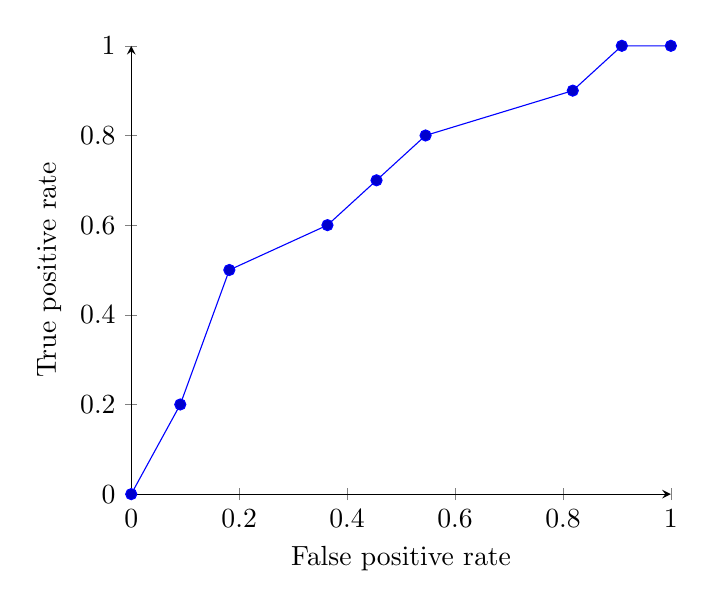
\begin{tikzpicture}
\begin{axis} [xlabel=False positive rate,
ylabel=True positive rate,axis x line=bottom,
axis y line=left]
\addplot coordinates { (0,0)(0.09090909090909091,0.2)(0.18181818181818182,0.5)(0.36363636363636365,0.6)(0.4545454545454546,0.7)(0.5454545454545455,0.7999999999999999)(0.8181818181818183,0.8999999999999999)(0.9090909090909093,0.9999999999999999) (1,1) };\end{axis}
\end{tikzpicture}\hfill \break
 AUC:0.7090909090909092
\hfill \break
\end{document}